\chapter{The new FASER Pre-Shower detector (14 pages)}

The motivation for the development of a completely new Pre-Shower detector for the FASER experiment at CERN has been outlined in \note{section ref}. This upgrade is driven by the need to enhance sensitivity to photonic final states, in particular to enable the detection of long-lived particles such as ALPs decaying into two photons. In addition to extending the reach of the FASER physics program, the new detector design could improve the discrimination power against background events and reinforce the robustness and reach of existing measurements. \\

This chapter presents a detailed description of the new Pre-Shower detector, from its smallest components to its integration into the full FASER detector. The discussion begins with a description of the ASIC, whose design is based on the knowledge acquired over the years at the University of Geneva by prototyping monolithic silicon pixel detectors for diverse applications. The ASIC is the smallest yet most essential piece of the detector as it digitises the position, time of passage and deposited charge of the traversing particle into a binary stream of data. The performance requirements for the ASIC are first presented, followed by a technical description of its architecture and the design choices made to satisfy the demanding constraints of the experiment. The data processing inside the ASIC is presented to highlight how the aforementioned parameters are extracted and digitised.  

The description then progresses to higher levels of integration. The Pre-Shower modules, each composed of six ASICs mounted on a single support structure, are introduced. These modules represent the basic building blocks of the system. A full detector plane is then formed by assembling twelve such modules, creating a scalable and modular structure. The mechanical layout of the full detector, including the positioning of the Pre-Shower planes and the absorber slabs used to initiate electromagnetic showers, is discussed and justified by the results of Monte Carlo simulations performed in \note{Cite Chiara's thesis} .

In the final part of the chapter, the focus shifts to the readout and control infrastructure. The architecture of the data acquisition chain is described, starting from the formatting of the digitised data and continuing through the transmission and processing of the data by the Logic Board (LB) and the Active Patch Panel (APP). The Pre-shower Interlock and Monitoring (PIM) module is introduced, and its functions are described.

Overall, this chapter aims to provide a comprehensive understanding of the design, functionality, and integration of the new Pre-Shower detector, a necessary upgrade of the initial FASER detector layout to enhance and reinforce its discovery potential.
	\clearpage 
	\section{Production ASIC Description }
	The development of the FASER Pre-Shower ASIC started in 2020 when a first 1.7$\times$2.6 mm$^2$ prototype with a matrix of 64 elongated hexagonal pixels with a footprint of 200$\times$50 $\mu$m$^2$, subdivided into five smaller matrices with different levels of integration of the frontend electronics as explained in \cite{FASER_proto0}. This ASIC was designed and produced in order to support the Pre-Shower upgrade proposal. In early 2021, the ASIC was tested and showed very satisfactory results in terms of gain and ENC. This study confirmed the feasibility of the integration of front-end elements inside the sensitive area, still complying with the requirements imposed. The results were published in the Journal of Instrumentation in late 2021 and can be found in \cite{FASER_proto0}. \\
	
	A second iteration before design and production of the final ASIC leading to a prototype of 15$\times$5.75 mm$^2$ with a matrix of 48$\times$128 (1536 total) pixels of regular hexagonal shape wit a \SI{65}{\micro\meter} side resulting in a pixel pitch of roughly \SI{100}{\micro\meter}. The pixel matrix is subdivided into three 16$\times$128 pixels Super-Columns (SCs), each subdivided into 8$\times$8 pixels Super-Pixels (SPs), each composed of 64 pixels. This architecture choice will later be discussed in section \note{section ref}. The purpose of this \textit{pre-production} prototype was to confirm the functionality of the front-end and digital electronics circuitry for the final ASIC, as well as studying the reliability of the power distribution over a large area ASIC and extract the production yield to infer what it would be for the larger \textit{production} ASIC. 
	
	The studies of this prototype have been published in \note{cite pre-prod paper} and helped refine the design of many components of the front-end circuitry, exhibiting large mismatches between pixel responses and current leakage, degrading the measurement of deposited. Additionally, the functionality of the ASIC readout was verified, and the production yield was estimated to be below 70\% and every ASIC exhibits a below 1\% % proportion of problematic pixels, more than acceptable from the imposed requirements. More details on the characteristics and testing of the \textit{pre-production} ASIC will be given in \note{section ref (if done)}. \\
	
	Finally, the design of the \textit{production} ASIC was completed in May 2023 and delivered in the laboratories of the University of Geneva after the wafers were thinned, back-processed and diced in collaboration with Micro-Packs in July 2024. In the following section, a description of the requirements of the ASIC performance is accompanied by a detailed description of the production ASIC. 
	
		\subsection{Requirements and Specifications}
		The design requirements on the FASER Pre-Shower \textit{production} ASIC are driven by the Monte Carlo studies performed on the production of ALPs and the topology of di-photon signals combined with simulations of the entire Pre-Shower detector in different layout configurations. The different requirements can often push the design choices in a different direction, and an overall robustness and design simplicity often dictate the direction of development. Some other specifications of the ASIC also meet requirements because of the previously acquired knowledge and widely tested structures in other projects by the design group of the University of Geneva. 
		
		\subsubsection{ASIC footprint}
		The \SI{20}{\centi\meter} aperture of the magnets of the FASER detector defines the total area the new Pre-Shower detector needs to cover. While from the Physics point of view, an ASIC as large as possible would represent the ideal case in terms of non-active area, from the electronics point of view, a smaller ASIC represent a larger yield as the probability of failure scales from one ASIC to the other to the power of the ratio in areas. Since ASICs are typically fabricated in rectangular shapes, the circular aperture must be instrumented using an array of identical rectangular sub-elements. As a result, some regions within the aperture may remain uninstrumented due to geometric constraints, while certain areas outside the nominal acceptance may inadvertently be covered. The size of the ASIC is then both driven by an optimised paving of the area available on a silicon wafer and by the need to provide modularity of the sub-elements of the Pre-Shower while keeping a total area leading to sufficient production yield. 
		
		\begin{figure}[h]
			\centering
			\includegraphics[width=0.9\textwidth]{files/ASIC_microscope}
			\caption{Microscope stitched image of the FASER \textit{production} ASIC. The sub-structures of the ASIC can be identified, such as the digital peripheries or contact metallic pads (rectangular grey pads on the top and bottom edges). The 13 vertical lines are the digital columns.}
			\label{im:ASIC_microscope}
		\end{figure}
		
		The \textit{production} ASIC has a total footprint of 22.15$\times$15.35 mm$^2$ with an active area covering 21.61$\times$14.36 mm$^2$ for a total of roughly 91\% of the ASIC area being active, hence resulting in 9\% of so-called "dead-area" mostly composed of the ASIC periphery. In addition, the dead area is also composed of 13 thin columns going across the ASIC's small side, also called the digital column. This structure has a pitch of roughly half the pixel pitch (\SI{60}{\micro\meter}) and contributes at the level of 3\% to the dead-area. A thoughtful assembly of ASICs together to pave the aperture of the magnet has to be made, it will be discussed in \note{ref to section on plane.} 
		The choice in size of the pixels composing the matrix was mainly driven by the already existing pixel design with hexagonal pixels with a side of \SI{65}{\micro\meter} for a pitch in both directions of roughly \SI{100}{\micro\meter}. The ALP Monte Carlo simulation exhibited a clear dependence on the rate of di-photon signals as a function of the required separation between showers initiated by the two photons, hence reducing the sensitivity reach. At first order, one can distinguish two different shower cores if there is at least one pixel separating the pixel containing the core of the showers, this leads to a separation between the photons of at least \SI{200}{\micro\meter}, for which the sensitivity reach is given as the second outermost line in figure \ref{im:reach_plot_detector}. The many different design challenges associated with a reduced pixel pitch did not justify a sufficient improvement of the performance in terms of sensitivity reach. 
		
		\subsubsection{High dynamic range}
		The performance of the new Pre-Shower lies in its ability to distinguish the cores of the electromagnetic showers produced by two close-by photons. As the photons have significant boost due to their very high energy, the core of the shower will remain narrow while the shower spread, depending mostly on secondaries with higher transverse momentum, will remain the same as it only depends on the amount of radiation length crossed and the critical energy in the medium in which the showers develops \cite{PDG}. In order to quantify the range of deposited charge in a single pixel, Monte Carlo simulations of incident photons with energies sampled from the ALP production simulations were realised. The studies are presented in \cite{Kotitsa_thesis}, and an interesting result is adapted in figure \ref{im:charge_per_plane_FASER}. The figure displays the distribution of the maximum charge recorded in a pixel (corresponding roughly to the charge of the core of the shower) for each plane in the FASER Pre-Shower.
		
		\begin{figure}[h]
			\centering
			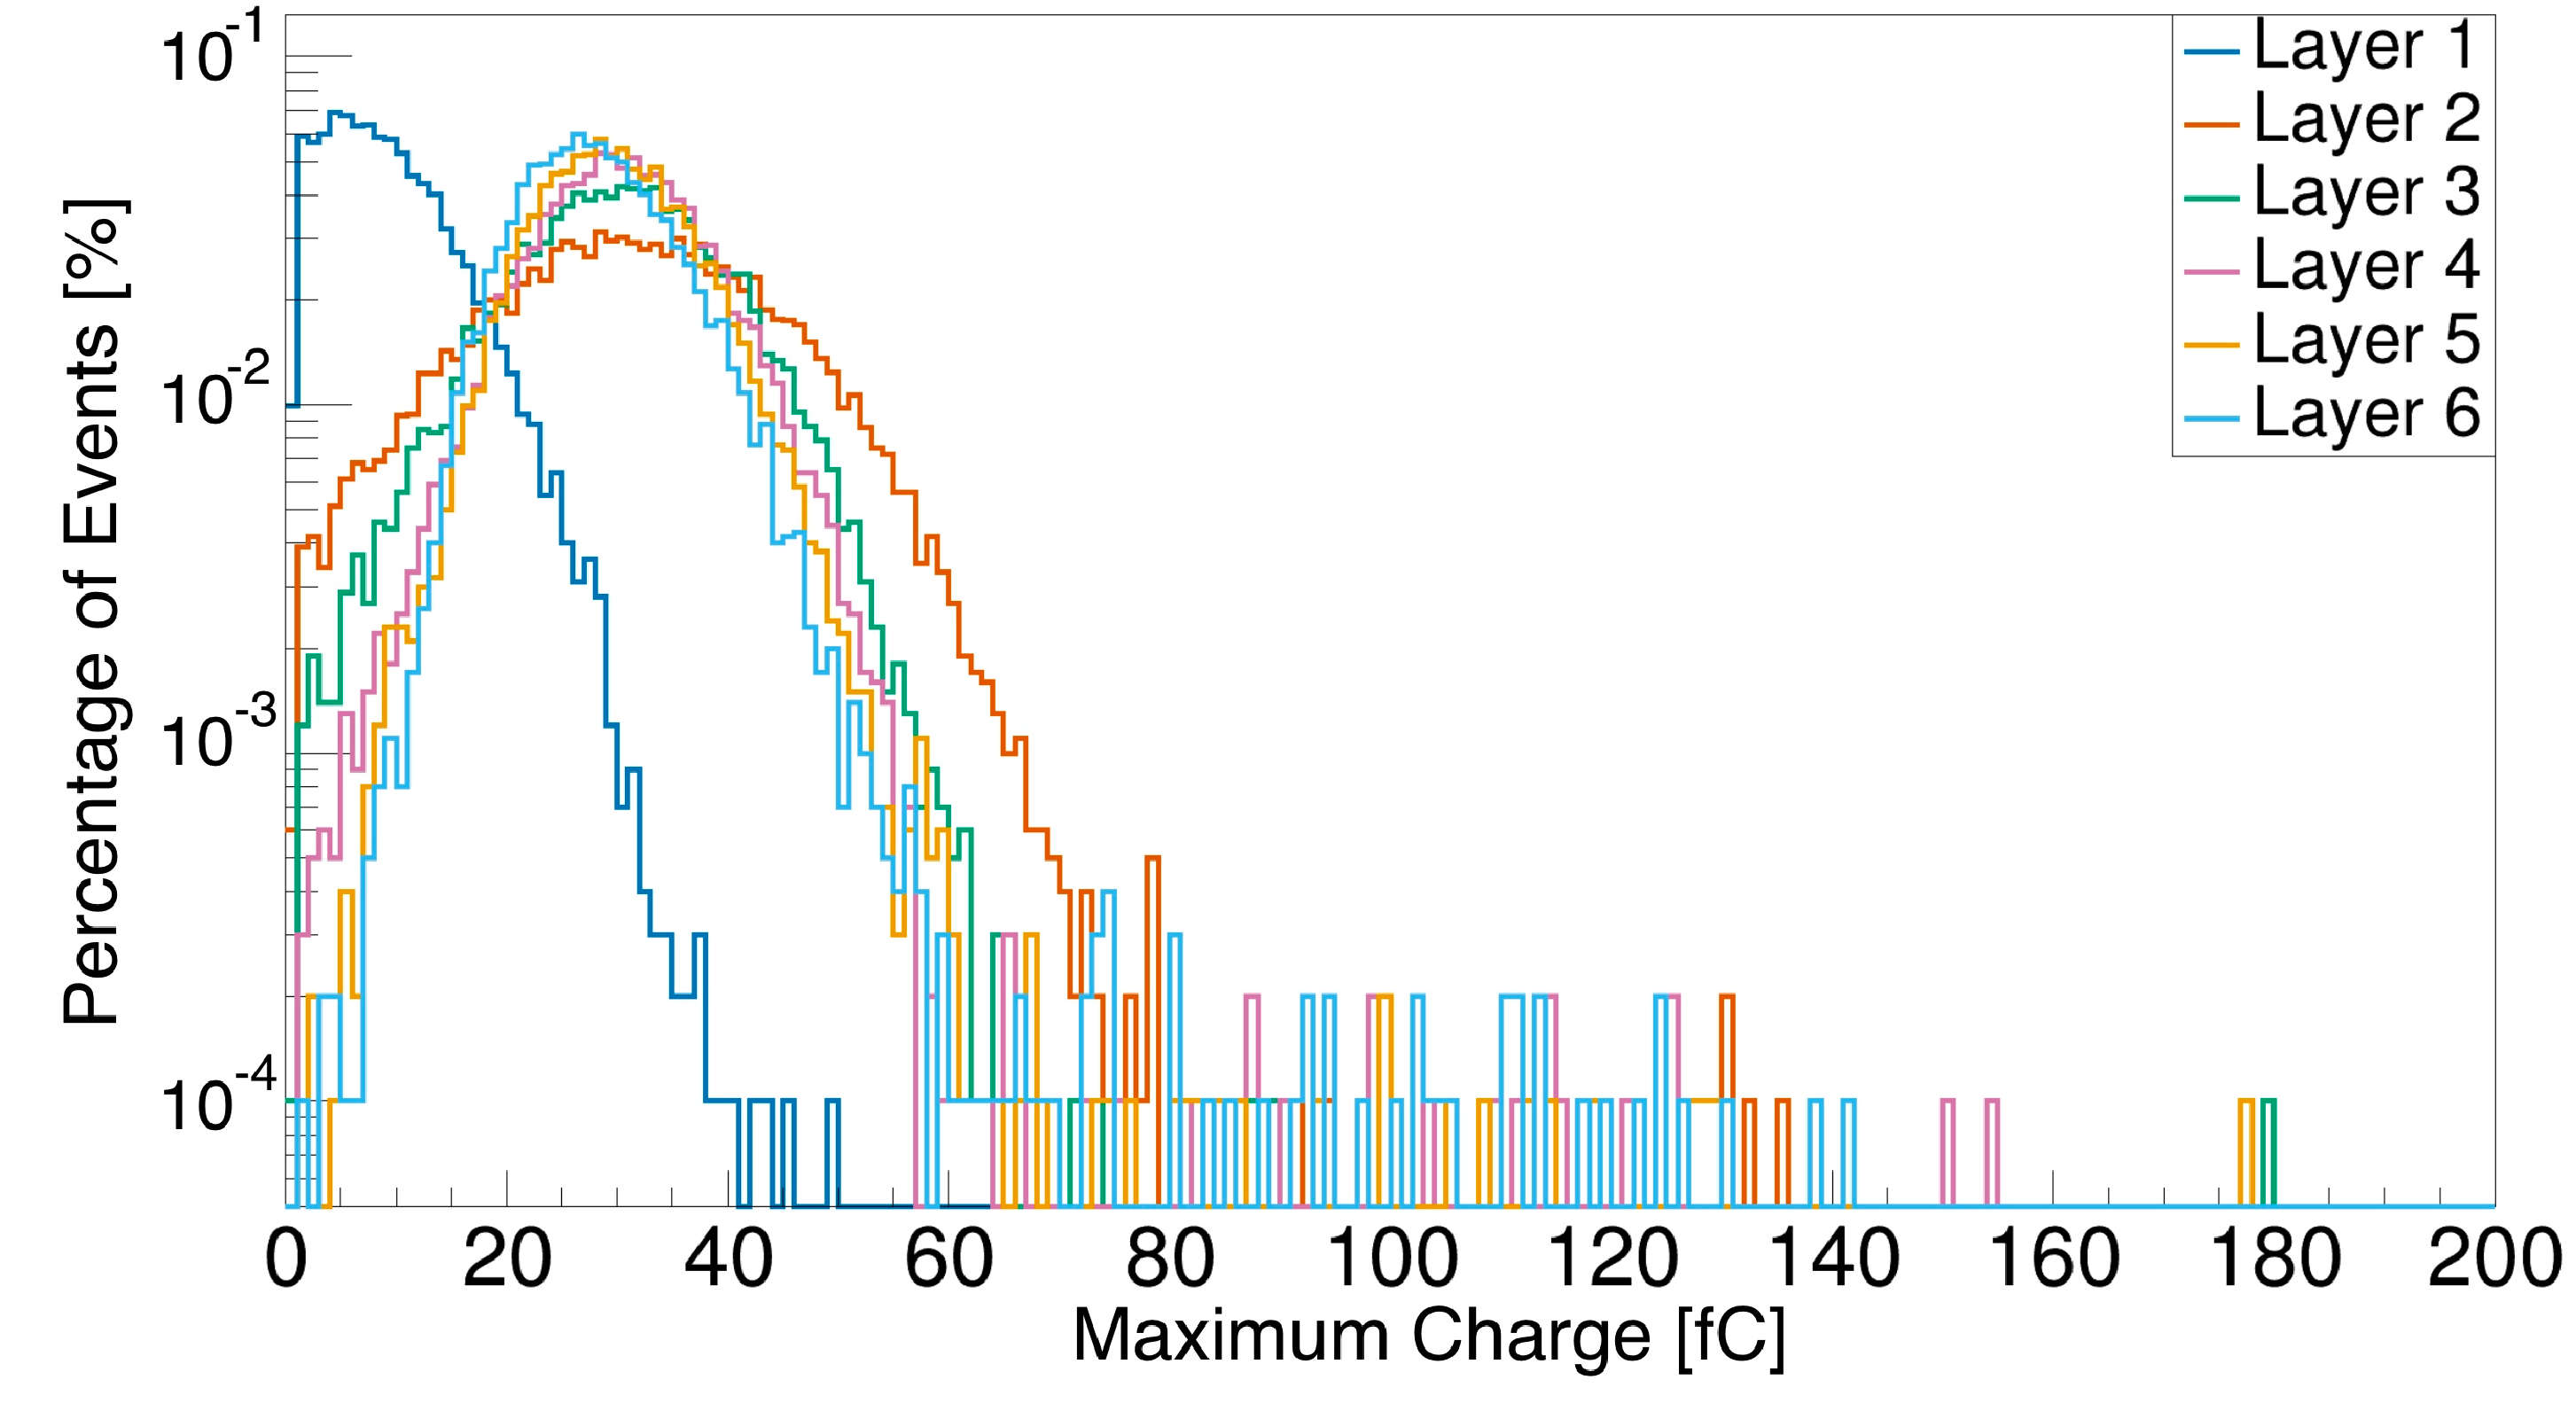
\includegraphics[width=0.8\textwidth]{files/charge_per_plane_FASER}
			\caption{Distribution of the maximum charge deposited in a single pixel across all the Pre-Shower detection planes for a total of 10k simulated events with two photons of \SI{1}{\tera\electronvolt} with a separation of \SI{500}{\micro\meter}. The maximum charge for all but the first plane roughly saturates between 60 and \SI{80}{\femto\coulomb} with very rare events reaching more than \SI{100}{\femto\coulomb}.}
			\label{im:charge_per_plane_FASER}
		\end{figure}
		
		The results of these simulations gave insight into what should be the upper limit of the charge measurement range. The \textit{production} ASIC hence has a dynamic range extending until a charge of \SI{65}{\femto\coulomb} for this reason. On the other hand, the lower limit of the dynamic range is constrained by the need to be sensitive to MIPs. Indeed, the planes of the preshower will need to be aligned among themselves to provide optimal position reconstruction performance and interpolation of shower core position across the detection planes. In the case of FASER, muons can be used as they provide very straight tracks with a very clean signature in the different detection planes, hence providing a very good alignment data sample. The mean energy deposition for a MIP in the thickness of silicon of the ASIC is \SI{0.3}{\femto\coulomb}. The dynamic range for the FASER \textit{production} ASIC was then designed to range between 0.5 and \SI{65}{\femto\coulomb}.
		
		\subsubsection{Fast Readout Time}
		A sufficiently fast readout time is essential in order to be sensitive to as many events as possible; any so-called "dead-time" could lead to losses in events, not optimal when looking for very rare processes. It was highlighted previously in \note{ref to background} that the most prominent source of background comes from high-energy muons, for which the rate was estimated to be \SI{0.5}{\hertz/\centi\meter\squared}. Simulations have shown that the typical multiplicity for muon events is roughly 1. The data pruning implemented on the ASIC limits the event size for an event with a single firing pixel to 3 kb, resulting in a time to send the data out of the ASIC of \SI{15}{\micro\second} at a 200 Mbps single data rate \cite{PreShower_TP}. Extrapolating the data rate for a full plane, since each half pane is readout independently, leads to a value of 405 kbps, rounded up to 450 kbps \cite{PreShower_TP} and leading to a readout time of \SI{2.25}{\milli\second} equivalent to as dead-time ratio of only 0.4\% for muons. Further details on the entire readout architecture and procedure will be given in \note{section ref}.
		
			The simulations also provided an estimate of the maximal occupancy of 1700 pixels for \SI{1}{\tera\electronvolt} photon events with a discrimination threshold of \SI{1}{\femto\coulomb}. To further limit the readout dead-time in the case of very rare photon events, the average number of bits to readout as a function of the number of active pixels was compared between a frame-based solution and a packet-based solution. The results are presented in Figure \ref{im:readout_data_size}, adapted from \cite{Martinelli_thesis}.
			
		\begin{figure}[h]
			\centering
			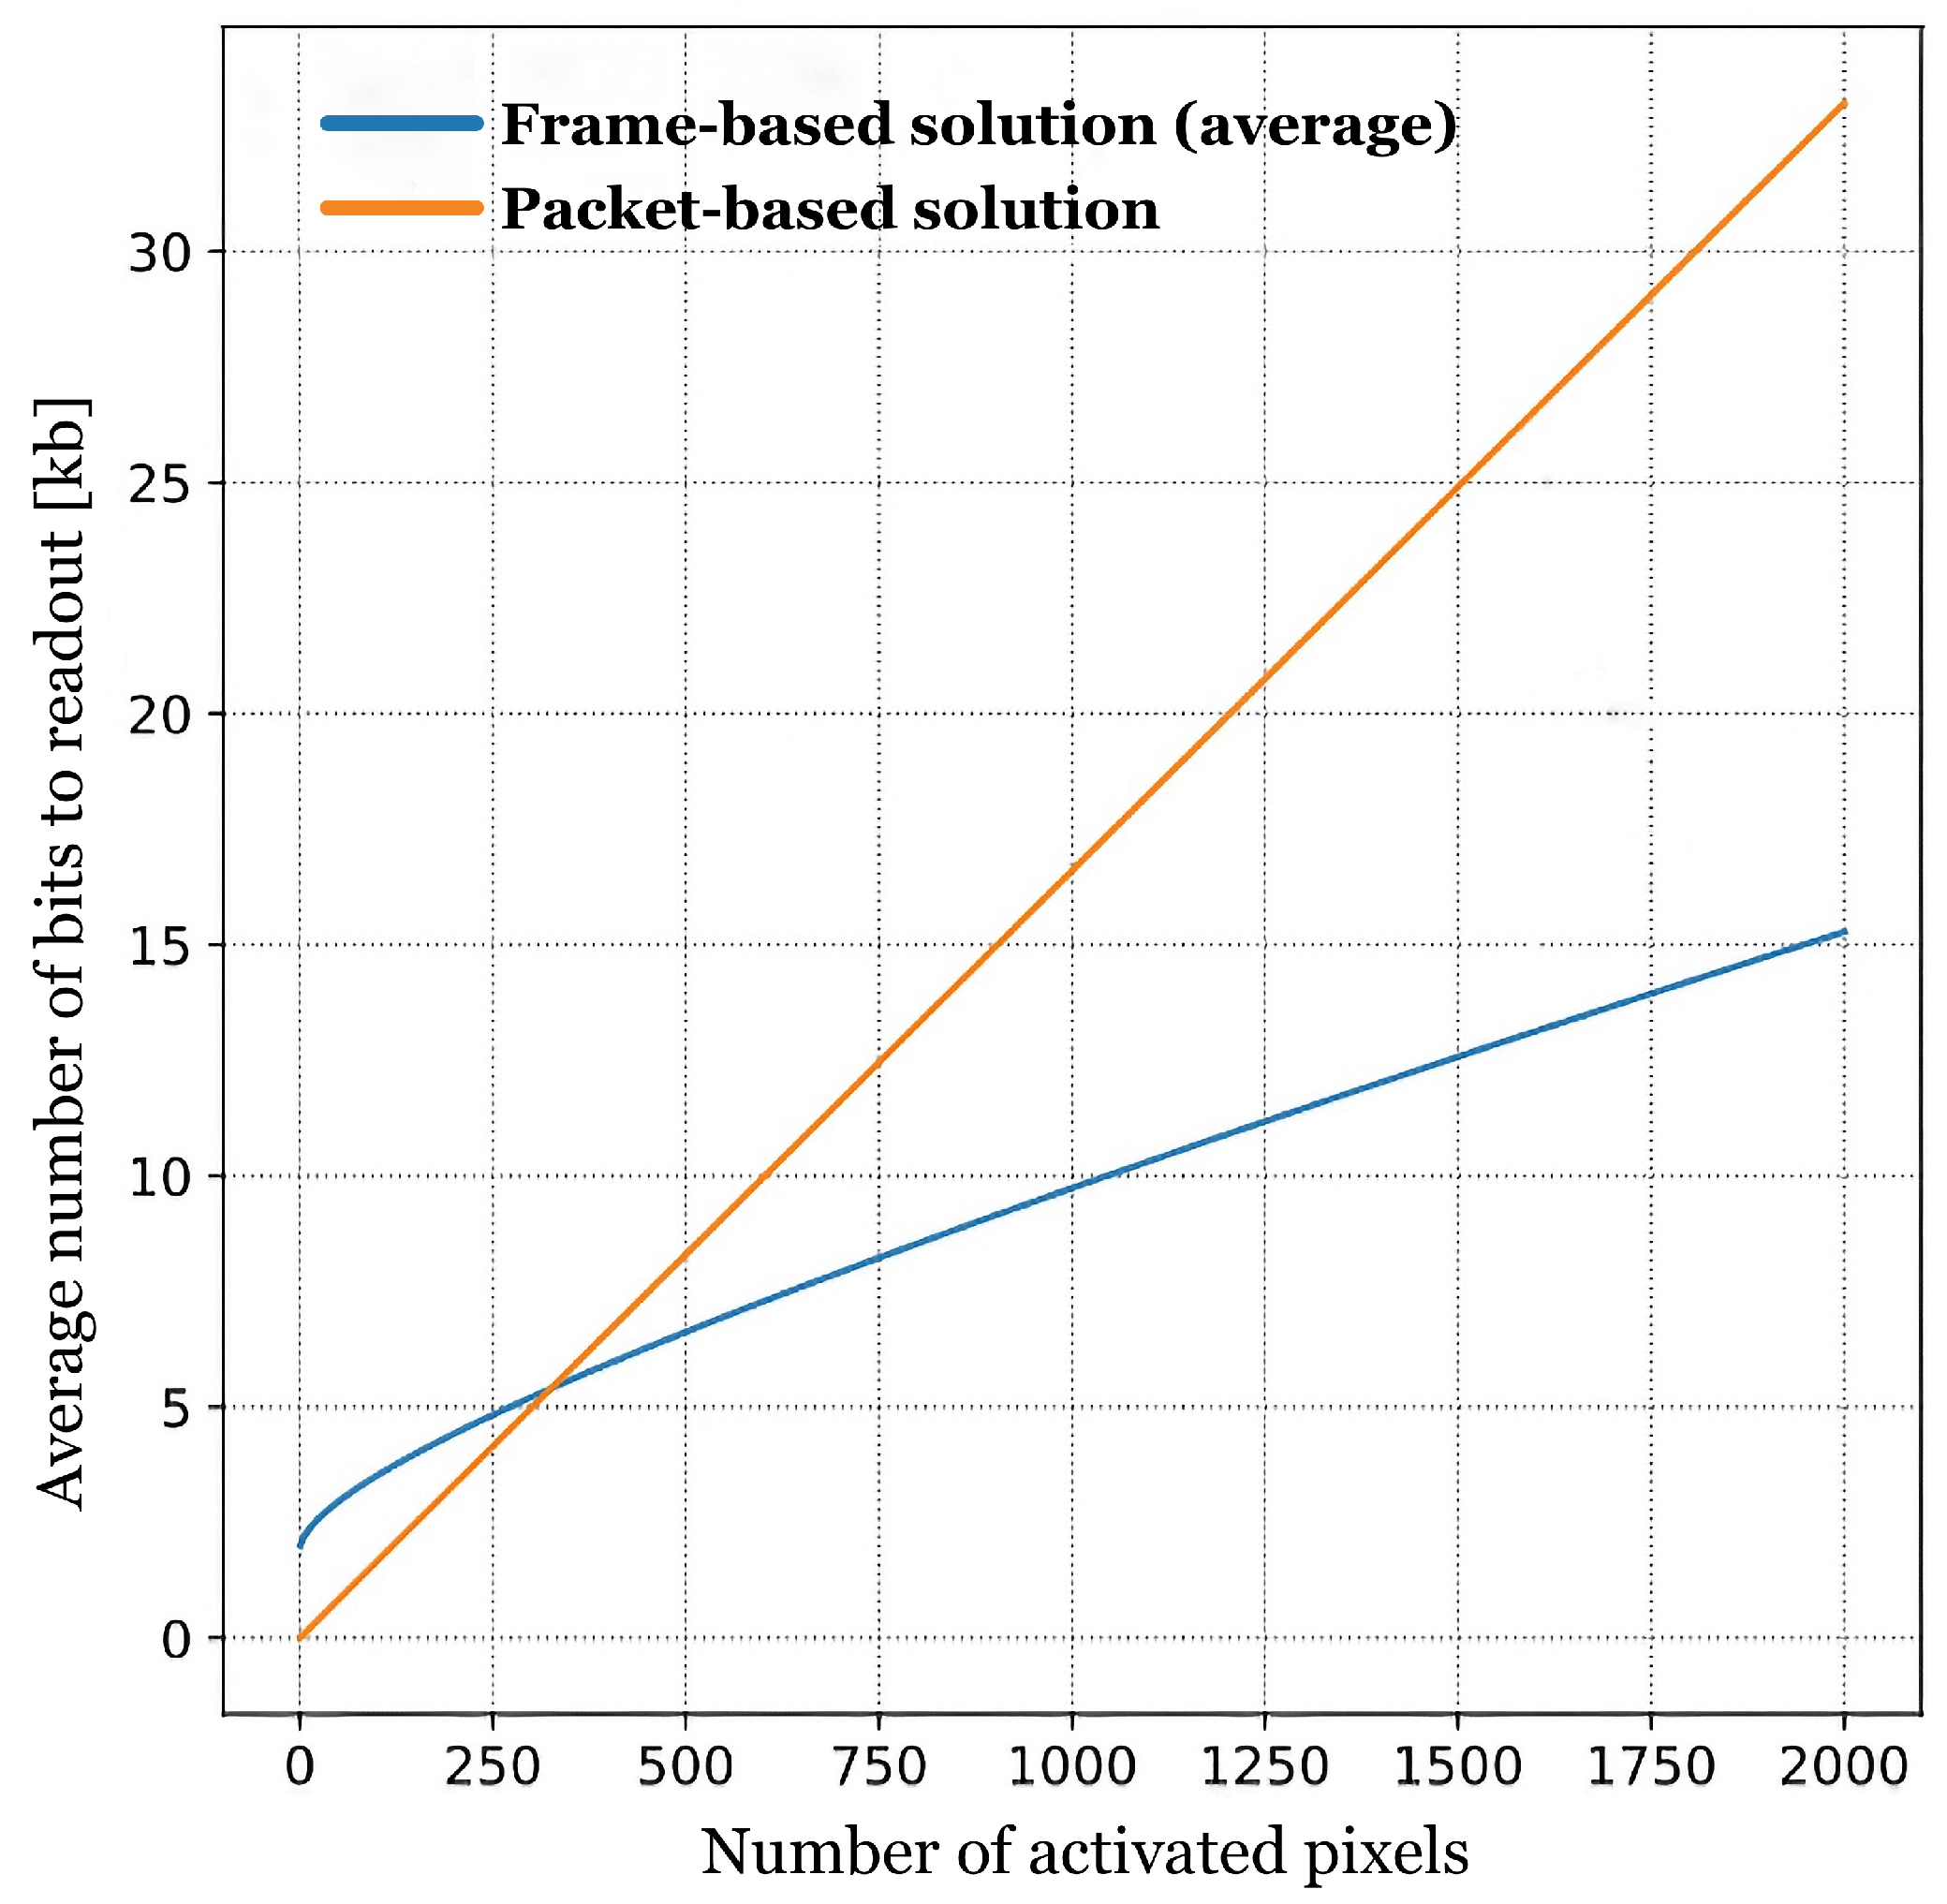
\includegraphics[width=0.7\textwidth]{files/readout_data_size}
			\caption{Comparison of the average number of bits to readout as a function of the number of activated pixels. For a number of activated pixels below 350, the frame-based solution produces a relatively lower while for large number of activated pixels such as 1700 (highest simulated occupancy), there is a difference of roughly 15 kb to be read out, leading to a reduction of almost a factor 2 in dead-time.}
			\label{im:readout_data_size}
		\end{figure}
		
		The packet-based solution offer a lighter solution for a number of activated pixels below 350 but for large number of activated pixels such has the maximal simulated occupancy of 1700 pixels, the frame-based architecture offers a much better solution. At such levels of occupancy, the difference in average number of bits to be readout is of the order of 15 kb, resulting in a reduction of the readout dead-time of a factor 2. This approach hence allows a suitable solution for reading out with high efficiency, photon events in the preshower. A more detailed discussion on the readout architecture will be provided in \note{ref to readout section}.
		
		\subsubsection{Low Power Operation and Thermal Management}
		The power consumption of the FASER \textit{production} ASIC is dominated by the current provided by the amplifier in the front-end electronics. By design, this nominal power density was estimated to be \power = \SI{150}{\milli\watt/\centi\meter\squared}. The digital power consumption is very local in time as it only pulls current when the chip is read out or configured, and its contribution is then neglected. The power consumption ($\mathcal{P}_{\text{C}}$) for a single ASIC can then be calculated as the product of the power density and the area of the active part of the ASIC, giving a value of $\mathcal{P}_{\text{C - ASIC}} \simeq $ \SI{0.470}{\watt}. A single module and plane would then respectively have a power consumption of $\mathcal{P}_{\text{C - Module}} \simeq $ \SI{2.8}{\watt} and $\mathcal{P}_{\text{C - Plane}} \simeq $ \SI{33.5}{\watt}.
		
		These values of power consumption comply with an active cooling using the existing water cooling system of the FASER detector, with a coolant temperature of \SI{15}{\celsius} \cite{PreShower_TP}. A follow-up discussion on the thermal cooling of planes will be given in \note{section ref (necessary to give?)}.
		
		
		The requirements on the ASIC architecture and performance have been defined through the study of the topology of di-photon events, the study of characteristics in terms of occupancy and deposited charge for photon events, but also by the study of muon background. The diverse constraints at the level of production design and services complement the requirements in defining the specifications of the FASER Pre-Shower \textit{production} ASIC.   
		
		
		\subsection{ASIC Architecture}
		The FASER Pre-Shower \textit{production} ASIC has an active area composed of a total of 26624 pixels arranged in a matrix of 208 columns and 128 rows. The ASIC is designed as a repetition of multiple substructures, going from the smallest to the largest (in size), one can identify the Pixel-Rows, the Super-Pixels and Super-Columns. Figure \ref{im:prodASIC_floorplan} shows the different elements and their arrangement in the ASIC. 
		
		\begin{figure}[h]
			\centering
			\includegraphics[width=1.0\textwidth]{files/floorplan}
			\caption{Microscope image of the FASER Pre-Shower \textit{production} ASIC with overlayed position of substructures. Super-pixels are shown only for one Super-Column, but they all have the same structure. Similarly, the structure of a single Super-Pixel is shown but the structure is identical for all Super-Pixels.}
			\label{im:prodASIC_floorplan}
		\end{figure}
		 
			\subsubsection{Pixel-Row}
			The Pixel-Row (PR) is the smallest building block of the ASIC after the smallest element, the pixel. The PR is composed of 8 pixels, each having its own front-end electronics inside the active area. The circuitry is composed of a biasing circuit, a test-pulse capacitor, the amplifier, a comparator for signal discrimination and an analog memory for storing the information relative to the amount of deposited charge. The PR is also composed of the masking logic, together with the memory control and the FAST-OR logic, located in the digital column. Figure \ref{im:pixel-row_logic} shows a conceptual diagram of the Pixel-Row architecture and routing. 
			
			\begin{figure}[h]
				\centering
				\includegraphics[width=0.8\textwidth]{files/Pixel-row_logic}
				\caption{Conceptual diagram of the Pixel-Row logic, highlighting the components located in the pixel active area and the digital column.}
				\label{im:pixel-row_logic}
			\end{figure}
			
			The pixels can be individually masked after the discrimination stage thanks to a single mask-control bit. The injection of the test-pulse into the test-pulse capacitor is also controlled by the mask-control bit and allows for the test-pulse distribution. The masking operation is performed at the level of the Super-Column by a long shift register mapped in the digital periphery as 128 arrays of 16 bits each, hence handling two Pixel-Rows per array. The masking map is given for a single row (made of two Pixel-Rows) for an odd-type and even-type SC in table \ref{tab:masking_map}.
			\begin{table}[h]
				\centering
				\renewcommand{\arraystretch}{1.2}
				\begin{tabular}{|c|c|c|c|c|c|c|c|c|c|c|c|c|c|c|c|c|}
				\cline{1-17}
				\multicolumn{17}{|c|}{Masking map for odd-type SC} \\ 
				\cline{1-17}
				15 & 14 & 13 & 12 & 11 & 10 & 9 & 8 & \hspace{4mm} & 7 & 6 & 5 & 4 & 3 & 2 & 1 & 0 \\
				\cline{1-17}
				\end{tabular}
				
				\vspace{4mm}
				\begin{tabular}{|c|c|c|c|c|c|c|c|c|c|c|c|c|c|c|c|c|}
				\cline{1-17}
				\multicolumn{17}{|c|}{Masking map for even-type SC} \\ 
				\cline{1-17}
				8 & 9 & 10 & 11 & 12 & 13 & 14 & 15 & \hspace{4mm} & 0 & 1 & 2 & 3 & 4 & 5 & 6 & 7  \\
				\cline{1-17}
				\end{tabular}
				\caption{Mapping of the mask-control bit for masking control. The number corresponds to their position in the shift register, while the location in the row is the physical position in the ASIC.}
				\label{tab:masking_map} 
			\end{table}
			
			The mapping shows the number as the index of the bit in the shift register, and the position within the row corresponds to the physical position in the ASIC. The mapping of the test-pulse injection is different and is presented for a single row in table \ref{tab:testpulse_map}.
			
			\begin{table}[h]
				\centering
				\setlength{\tabcolsep}{4pt}
				\begin{tabular}{|c|c|c|c|c|c|c|c|c|c|c|c|c|c|c|c|c|}
				\cline{1-17}
				\multicolumn{17}{|c|}{Masking map for odd-type SC} \\ 
				\cline{1-17}
				15 & 11 & 13 & ~9 & 11 & 13 & ~9 & 15 & \cellcolor{darkred} & ~0 & ~6 & ~2 & ~4 & ~6 & ~2 & ~4 & ~0 \\
				\cline{1-17}
				\end{tabular}
				
				\vspace{4mm}
				\begin{tabular}{|c|c|c|c|c|c|c|c|c|c|c|c|c|c|c|c|c|}
				\cline{1-17}
				\multicolumn{17}{|c|}{Masking map for even-type SC} \\ 
				\cline{1-17}
				~8 & 14 & 10 & 12 & 14 & 10 & 12 & ~8 &\cellcolor{darkred} & ~7 & ~3 & ~5 & ~1 & ~3 & ~5 & ~1 & ~7  \\
				\cline{1-17}
				\end{tabular}
				\caption{Mapping of the mask-control bit for test-pulse control. The number corresponds to their position in the shift register, while the location in the row is the physical position in the ASIC. The central separation shows the digital column.}
				\label{tab:masking_map} 
			\end{table}
			
			Not all the mask-control bits control the injection of the test-pulse. Only one out of two is used, resulting in every bit controlling simultaneously the injection in two non-adjacent pixels. While testing a wise combination of the mask-control bits, nevertheless enabling testing the pixel's response to test-pulse one-by-one. 
				
			\subsubsection{Super-Pixel} 
			Every Super-Column is subdivided into 8 Super-Pixels, all identical and numbered from 0 to 7 from bottom to top of the ASIC. Each SP is composed of 256 pixels arranged in a matrix of 16 rows and 16 columns of pixels and represents the basic block of the readout logic. Super Pixels have their bias generation circuit to avoid mismatch due to voltage drop over the power supplies. The circuitry for the measurement of the charge deposited in every pixel is also defined at the SP level and is composed of a 256:1 multiplexer (MUX) and a 4-bit flash Analog to Digital Converter (flash-ADC) made of 15 comparators referred to equally spaced and increasing thresholds. Figure \ref{im:SuperPixel_logic} presents a conceptual diagram for the architecture and routing of the Super-Pixel. 
			\begin{figure}[h]
				\centering
				\includegraphics[width=1.0\textwidth]{files/SuperPixel_logic}
				\caption{Conceptual diagram of the Super-Pixel logic. The FAST-OR connections are referred to as those of an even-type SC. }
				\label{im:SuperPixel_logic}
			\end{figure}
			
			 The FAST-OR generation is also located at the SP level and is then sent to the digital periphery for triggering the readout but also to 3 TDC channels associated to each line for time digitisation. The FAST-OR mapping is cyclic every 3 pixel rows and is the same for any SP within a SC. Figure \ref{im:FastOR_map} shows the mapping for 3 pixels rows for both SC types. 
			
			\begin{figure}[h]
				\centering
				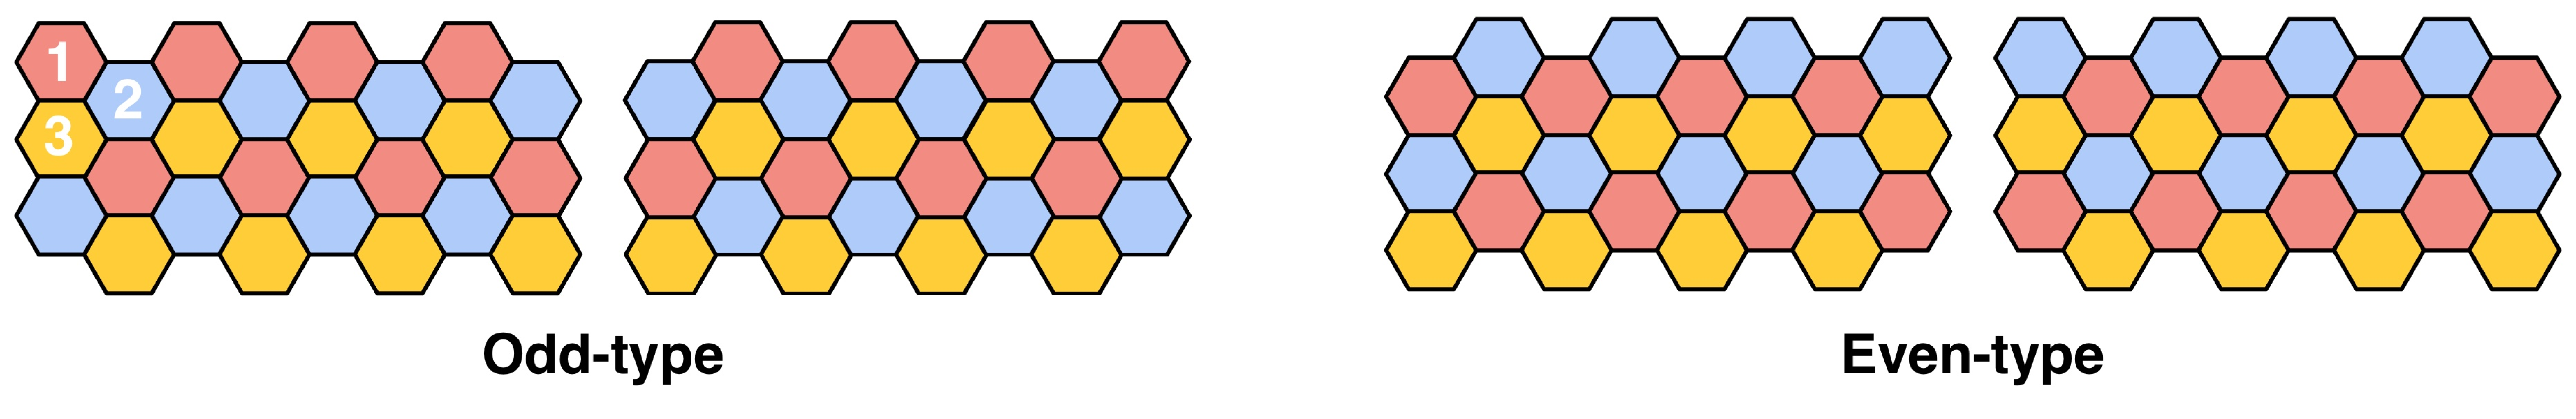
\includegraphics[width=1.0\textwidth]{files/FastOr_map}
				\caption{Mapping of the FAST-OR lines for 3 consecutive pixel rows for an odd-type SC (left) and an even-type SC (right). Each colour represents a FAST-OR line. At the level of the SP, all the lines from each pixel of the same colour is put in OR and the resulting signal is sent to the digital periphery for triggering and to the TDCs for precise time digitisation.}
				\label{im:FastOR_map}
			\end{figure}
			
			
			\subsubsection{Super Column} 
			The ASIC is composed of 13 Super Columns (SC), which can further be divided into two subgroups: the odd-type and even-type SCs. The SC numbering start from the left hand side of the ASIC (see figure \ref{im:prodASIC_floorplan}) with the leftmost one being an odd-type SC. The distinction between odd-type and even-type is essential as the routing of the pixels is different, meaning that one has to keep in mind how pixels are geographically mapped to their respective configuration and readout lines in each case. \note{Only for the odd/even convention the numbering start from 1, when identifying the SC in the matrix the number starts from 0.} Each SC is an independent building block of the ASIC, their configuration and readout is done separately and are all connected to the digital periphery. Nevertheless, they all share the same alimentations in terms of low voltages. 
				
			The SC is made of 2048 pixels arranged in a matrix of 128 rows and 16 columns of pixels and is split in half by the digital column, a \SI{60}{\micro\meter} wide non active part going from top to bottom of the SC representing roughly 3\% of the total area of the SC. This portion of the SC is dedicated to the various lines needed for powering, configuration of the pixels and readout.
			Each SC possesses its own time digitisation block composed of a 24-channel Time to Digital Converters (TDC). The mapping of the TDC channels to the FAST-ORs of each SP is different for odd-type and even-type SC and is given by table \ref{tab:tdc_fastor_map}
	
			\begin{table}[h]
				\definecolor{fo1}{HTML}{F28B82} 
				\definecolor{fo3}{HTML}{FFCD38} 
				\definecolor{fo2}{HTML}{AECBFA} 
    			\centering
    			\setlength{\tabcolsep}{4pt}
    			\scriptsize
    			\begin{tabular}{|c|*{24}{c|}}
    				\hline 
    				\multicolumn{25}{|c|}{\textbf{Mapping for even-type SC}} \\
       			 	\hline
        			\textbf{TDC Channel} 
        			& 0 & 1 & 2 & 3 & 4 & 5 & 6 & 7 & 8 & 9 & 10 & 11 
        			& 12 & 13 & 14 & 15 & 16 & 17 & 18 & 19 & 20 & 21 & 22 & 23 \\
        			\hline
        			\textbf{FAST-OR ID} 
        			& \cellcolor{fo2}2 & \cellcolor{fo1}1 & \cellcolor{fo3}3 & \cellcolor{fo2}2 & \cellcolor{fo3}3 & \cellcolor{fo3}3 & \cellcolor{fo2}2 & \cellcolor{fo1}1 & \cellcolor{fo3}3 & \cellcolor{fo2}2 & \cellcolor{fo1}1 & \cellcolor{fo3}3 
        			& \cellcolor{fo2}2 & \cellcolor{fo3}3 & \cellcolor{fo2}2 & \cellcolor{fo1}1 & \cellcolor{fo3}3 & \cellcolor{fo1}1 & \cellcolor{fo2}2 & \cellcolor{fo3}3 & \cellcolor{fo1}1 & \cellcolor{fo2}2 & \cellcolor{fo3}3 & \cellcolor{fo1}1 \\
        			\hline
        			\textbf{Super Pixel ID} 
       			 	& 0 & 1 & 1 & 2 & 3 & 3 & 4 & 5 & 5 & 6 & 7 & 7 
       				& 7 & 6 & 6 & 5 & 4 & 4 & 3 & 2 & 2 & 1 & 0 & 0 \\
        			\hline
    			\end{tabular}
    
    			\vspace{4mm}
    
    			\begin{tabular}{|c|*{24}{c|}}
       				\hline 
    				\multicolumn{25}{|c|}{\textbf{Mapping for odd-type SC}} \\
    				\hline
        			\textbf{TDC Channel} 
        			& 0 & 1 & 2 & 3 & 4 & 5 & 6 & 7 & 8 & 9 & 10 & 11 
        			& 12 & 13 & 14 & 15 & 16 & 17 & 18 & 19 & 20 & 21 & 22 & 23 \\
        			\hline
        			\textbf{FAST-OR ID} 
        			& \cellcolor{fo2}2 & \cellcolor{fo3}3 & \cellcolor{fo1}1 & \cellcolor{fo2}2 & \cellcolor{fo3}3 & \cellcolor{fo1}1 & \cellcolor{fo2}2 & \cellcolor{fo3}3 & \cellcolor{fo1}1 & \cellcolor{fo2}2 & \cellcolor{fo3}3 & \cellcolor{fo1}1 
        			& \cellcolor{fo2}2 & \cellcolor{fo1}1 & \cellcolor{fo3}3 & \cellcolor{fo2}2 & \cellcolor{fo1}1 & \cellcolor{fo3}3 & \cellcolor{fo2}2 & \cellcolor{fo1}1 & \cellcolor{fo3}3 & \cellcolor{fo2}2 & \cellcolor{fo1}1 & \cellcolor{fo3}3 \\
        			\hline
        			\textbf{Super Pixel ID} 
        			& 0 & 1 & 1 & 2 & 3 & 3 & 4 & 5 & 5 & 6 & 7 & 7 
        			& 7 & 6 & 6 & 5 & 4 & 4 & 3 & 2 & 2 & 1 & 0 & 0 \\
        			\hline
    			\end{tabular}
    			\caption{Mapping between TDC channels, FAST-OR ID inputs, and Super-Pixel IDs for even-type (top) and odd-type (bottom) SCs.}
    			\label{tab:tdc_fastor_map}
			\end{table}
			
			The TDCs are composed of a 7-block ring oscillator and 24 counters, all latched separately. The counters corresponds to the 24 channels mentioned previously and are composed of a 7-bit fractional data, given by the status of the ring oscillator, and a 11-bit counter data. The TDC also possesses a reference channel with a 7-bit fractional data and 6-bit counter data, used to measure the period between two clock cycles.
			Next to the TDC block is located, before the digital periphery, the End-Of-Column (EOC) logic block responsible for communication between the pixel matrix and the periphery, it handles both communication and configuration for the entire SC.   
		
		\subsection{Signal Digitisation and Readout}
		From the moment a particle crosses the active area of a pixel and deposits a sufficient amount of charge such that the level at output of the amplifier is higher than the threshold level in the discriminator, a sequence of operations is performed by the ASIC in order to digitise the information relative to the detection of that particle. The information regarding the position, time and charge deposited is then formatted into a binary bitstream in output of the ASIC. In the following section, a presentation of the ASIC operations followed by the description of the structure of the bitstream will be presented. 
		
			\subsubsection{Digitisation}
			A conceptual description of the circuitry responsible for the digitisation of the information relative to the passage of the particle in a pixel. The different steps can be listed as follows: 
			\begin{enumerate} [1.]
				\item The discriminator, located inside the comparator block, outputs a digital signal whose length in time is proportional to the logarithm of the charge deposited in the pixel. This signal is compared to the value of the mask-control bit for that pixel.
				\item If the pixel in un-masked, two copies of the signals are generated. 
				\begin{enumerate}[(i)]
					\item A first copy asynchronously goes to the FAST-ORs, which are then connected to the TDCs at the end of the SC. This signal will latch the corresponding TDC channel, resulting in the measure of the time of arrival. 
					\item A second copy is sent to the memory control block which charges the analog memory with a constant (configurable) current for a time proportional to the duration of the digital signal, i.e. the ToT of the output of the amplifier. The information relative to the charge deposited in the pixel's active area is now stored as a charge on a capacitor, the analog memory.   
				\end{enumerate}
				
				The readout process is initiated when the output of the OR is also sent as a trigger signal to the EOC which sends it to the digital periphery. At the same time, any other occurence in the trigger from any SC is masked so that any particle crossing the ASIC while in its readout phase will be lost. 
			
				\item The first phase of the readout consists in waiting enough time for the analog memories to be fully charged. The waiting time is configurable such that if corresponds to $ 4 \times readout\_config + 2 \textit{ clock cycle}$, where $readout\_config$ is an 8-bit register delaying the start of the readout in units of 2 clock cycles. In parallel, a calibration and reference signal is sent to the TDC. Once the waiting time is finished, the digital periphery starts polling the data from the SC sequentially. 
				\item If a SC has a hit, the EOC will send the ADC and TDC data.
				\begin{enumerate}[(i)]
					\item The SC sets the address in the MUX so it connects to the pixel with ID 0 in every Super-Pixel. 
					\item A waiting time know as $pause\_ADC$ configurable through the last 3 bits of an 8-bit register named $config\_global$, is given to the MUX to change address and for flash-ADC to measure the charge of the analog memory. The SC reads the ADC value and transmit it (if there is any) for every SP. 
					\item The SC set the address of the MUX so it connects to the pixel with ID 1 in every Super-Pixel.
					\item The sequence is repeated until the address of the MUX is set so it connects to pixel 255.    
				\end{enumerate}
			
				\item The SC gets the TDC data and sends it to the digital periphery. 
				\item This sequence is repeated until all of the SC with at least one pixel firing are read. 
				\item Once the last SC was readout, a waiting time corresponding to 100 clock cycles is imposed before unmasking the trigger signals from columns, a reset to the analog memories is sent for a time equivalent to 20 clock cycles. The ASIC is ready for the next readout phase. 
			\end{enumerate}
		
			One could realise that both the time and charge information has been digitised and sent in output of the ASIC, but it is nowhere specified how the information relative to the position has been digitised. This information is actually encoded in the order in which the pixels are read. Since the MUX probes every pixel in a specific order it is possible to build a map of the physical position of the pixel inside the matrix as a function of the order of the pixel information in the output data. The mapping is different for an odd-type and even-type SC and is presented in table \ref{tab:output_pixels_map} for the pixel row the closest to the digital periphery. 
		
		
			\begin{table}[h]
				\centering
				\setlength{\tabcolsep}{3pt}
				\begin{tabular}{|c|c|c|c|c|c|c|c|c|c|c|c|c|c|c|c|c|}
				\cline{1-17}
				\multicolumn{17}{|c|}{Output map for odd-type SC} \\ 
				\cline{1-17}
				~56~ & ~48~ & ~40~ & ~32~ & ~24~ & ~16~ & ~~8~ & ~~0~ & \cellcolor{darkred} & 1024 & 1032 & 1040 & 1048 & 1056 & 1064 & 1072 & 1080 \\
				\cline{1-17}
				\end{tabular}
			
				\vspace{4mm}
				\begin{tabular}{|c|c|c|c|c|c|c|c|c|c|c|c|c|c|c|c|c|}
				\cline{1-17}
				\multicolumn{17}{|c|}{Output map for even-type SC} \\ 
				\cline{1-17}
				~~0~ & ~~8~ & ~16~ & ~24~ & ~32~ & ~40~ & ~48~ & ~56~ & \cellcolor{darkred} & 1080 & 1072 & 1064 & 1056 & 1048 & 1040 & 1032 & 1024  \\
				\cline{1-17}
				\end{tabular}
				\caption{Mapping of order in which pixel information is readout and sent in output of the ASIC. The number corresponds to their position in the output data while the location in the row is the physical position in the ASIC. The central separation shows the digital column.}
				\label{tab:output_pixels_map} 
			\end{table}	
		
			In order to obtain the missing 15 rows within the super pixel, one has to remember that because of the 8 SP and 8 pixel per Pixel-Row, the periodicity of this pattern is 64. For the second closest SP to the digital periphery, one can simply use the map for the closest SP and shift every value by 1 index. The position of the pixel hit, is then encoded in the position of the data of the pixel in the output data. 
		
			\subsubsection{Readout and Bitstream Structure}
		
			The digital logic was designed to operate at a clock frequency of \SI{200}{\mega\hertz} so that each LVDS output provides a bandwidth of 200 Mbps. As a consequence of the different steps presented above, the ASIC will compose a bitstream, collecting and arranging in a structured manner all of the digitised data mentioned previously. Some additional bits are also present, such as so-called flags, indicating whether or not certains entities had a pixel firing or not. Moreover, since the ASIC continuously sends the data, the waiting time also represent part of the bitstream, at the exception of the initial and final waiting time, respectively before starting readout and once it is finished. The most comprehensive presentation of the structure of the bitstream is given in figure \ref{im:bitstream_structure}.

			\begin{figure}[h]
				\centering
				\includegraphics[width=0.95\textwidth]{files/bitstream_structure}
				\caption{Expected bitstream from the readout of the FASER Pre-Shower \textit{production} ASIC. The schematic representation shows the internal loops over SCs, SPs, pixels and TDC channels. The bits in red are used as references to identify the different steps in the readout. After the end of column flag, some possibles zeroes could be added by the ASIC but are to be ignored. }
				\label{im:bitstream_structure}
			\end{figure}
			
			This sequence is used as a reference for implementing the data decoding routines to transform the encoded data into usable variables such as pixel hit position in the matrix, charge associated to the hits and time of arrival. More details about the data conversion procedure will be given in \note{section ref}. 
		\clearpage
		\subsection{Configuration and Slow Control}
		The Slow Control of the ASIC for configuration relies on an SPI-like protocol with four single-ended lines: SPI$\_$clk for the clock signal, only sent during configuration and 0 polarity, SPI$\_$CS for the Chip Select, active low, SPI$\_$MOSI for sending commands and SPI$\_$MISO for reading back the data from the registers. The configuration commands are always 20-bit long. The SPI$\_$CS line allows for configuration of multiple ASICs in parallel but the command also incorporates a chip ID to address a specific ASIC. The SPI$\_$clk runs at a frequency of \SI{20}{\mega\hertz}. The commands structure is given in figure \ref{im:command_structure}. 
		
		\begin{figure}[h]
			\centering
			\includegraphics[width=1.0\textwidth]{files/command_structure}
			\caption{Command structure for the configuration of ASIC parameters through the SPI interface. Data are sent from left to right, Most Significant Bit (MSB) first.}
			\label{im:command_structure}
		\end{figure}
		
		The command is composed of: 
		\begin{enumerate}
			\item \textbf{S1}: Used for different types of commands: 
			\begin{itemize}
				\item $\left[00\right]$ writes data through SPI, the value in DATA[7:0] is written in the register located at ADDRESS[5:0],
				\item $\left[11\right]$ is a reset,
				\item $\left[10\right]$ is to push the masking configuration to the SC,
				\item $\left[01\right]$ to read on the SPI$\_$MISO the content of the register written by SPI$\_$MOSI.
			\end{itemize} 
			\item \textbf{ADDRESS}: The address pointing to the position of the register.
			\item \textbf{CHIP ID}: A value that is hard-coded by wire-bonds on the ASIC, if the hard-coded value does not correspond to the value in the command, this later is ignored. 
			\item \textbf{S2}: This bit, associated to the 3 Least Significant Bits (LSBs) of ADDRESS[5:0] are used to build the SC ID. When writing in registers, these are the same for every SC and so this feature is not used. Vice versa, when sending the masking command, the control is at the level of the SC, there is no register address and so the 6-bit address can be used as described.
			\item \textbf{DATA}: The 8-bit content to be written in the registers. 
		\end{enumerate}
		
		The performance of the ASIC in terms of deposited charge sensitivity and dynamic range of the charge measurement are controlled through a set of registers. Som other registers are used to configure the digital periphery. The ASIC has a total of 16 programmable 8-bit registers whose names and address and collect in table \ref{tab:SPI_parameters}
		
		\begin{table}[h!]
			\centering
			\begin{minipage}[t]{0.48\textwidth}
			\centering
				\begin{tabular}{|c|l|}
					\hline
					\textbf{Address} & \textbf{Register} \\ \hline
					000101 & bias\_preamp \\ \hline
					000110 & bias\_feedback \\ \hline
					000111 & bias\_disc \\ \hline
					001000 & bias\_idle \\ \hline
					001001 & bias\_LVDS \\ \hline
					001010 & bias\_load \\ \hline
					001011 & bandgap\_config \\ \hline
					001100 & bias\_testpulse \\ \hline
				\end{tabular}
			\end{minipage}
			\hfill
			\begin{minipage}[t]{0.48\textwidth}
			\centering
				\begin{tabular}{|c|l|}
					\hline
					\textbf{Address} & \textbf{Register} \\ \hline
					001101 & threshold\_set \\ \hline
					011101 & threshold\_offset \\ \hline
					010011 & bias\_pixel \\ \hline
					110010 & testpulse\_delay \\ \hline
					011110 & config\_global \\ \hline
					011111 & readout\_config \\ \hline
					000010 & programming\_word \\ \hline
					000011 & TDC\_config \\ \hline
				\end{tabular}
			\end{minipage}

			\caption{5-bit address of the registers and their name for reference.}
			\label{tab:SPI_parameters}
		\end{table}
		
		The registers all have a specific impact on the ASIC performance and behaviour but for simplicity, it is possible to group them into sub-categories, hence providing a clearer overview of their role:  
		\begin{enumerate}[i)]
			\item \textbf{Analogic}: The \textit{bias$\_$preamp}, \textit{bias$\_$feedback} and \textit{bias$\_$disc} are registers of the analog part of the front-end. The bias of the preamplifier sets the gain of the amplifier itself while the feedback bias regulates the gain bandwidth product. A higher bias\_preamp value gives a better gain and a high feedback value makes the amplifier faster at the cost of having reduced gain. Both are acting on the sensitivity of the front-end. The discriminator bias, controls the current used to switch between the different output levels of the discriminator, the higher the bias current and te faster it will switch. The value of the discriminator bias can't reach the highest values of the registers without sending the pixel in oscillation through capacitive coupling due to high transient currents. \\ Additionally, \textit{threshold$\_$set} and \textit{threshold$\_$offset} are used to determine in the discriminator, the level with which the output of the amplifier is compared. The effective threshold is the sum of the value given by each register (hence making it a 9-bit register instead of an 8-bit register). 
			\item \textbf{Analog memories}: The \textit{bias$\_$load}, \textit{bias$\_$idle}, \textit{readout$\_$config} and the 3 MSB of \textit{config$\_$global} are registers acting on the charge measurement through the analog memories. The ASIC is operated in two modes: measure mode and readout mode. When in idle the ASIC is in measure mode and, when a pixel is hit, the analog memories are charged with a current whose value is set through the \textit{bias$\_$load} register. The memories are charged while the ASIC in measure mode, it has to wait a time defined by the \textit{readout$\_$config} register, before switching into readout mode. When the memory is connected to the ADC through the MUX, since the MUX has its own parasitic resistance and capacitance, a waiting time is required before reading the status of the flash-ADC. This time is controlled by the 3 MSB of \textit{config$\_$global}, also known as \textit{pause$\_$adc}. Once the readout is finished and the ASIC is back in measure mode, the analogue memories are reset and the \textit{bias$\_$idle} makes sure that there is no leakage of current charging the memories from the memory control while in idle. 
			\item \textbf{Calibration}: The \textit{bias$\_$testpulse}, \textit{testpulse$\_$delay}, \textit{bandgap$\_$config} and \textit{TDC$\_$config} are registers used for calibration of the ASIC. The testpulse is a circuit that is used to inject a quantified amount of charge in the pixel, by charging a capacitor connected in parallel to the pixel. The testpulse is composed of a switch, which determines if the charge is injected or not in the pixel, controlled by the LSB of \textit{bandgap$\_$config}. A second switch is used for the injection, it goes from two different voltage levels, of which one is set by the value of the register \textit{bias$\_$testpulse}, which defines the amount of charge injected, and the frequency at which the switch changes position is defined by the value of \textit{testpulse$\_$delay}. It is interesting to note that is the delay on the testpulse is set to 0, this is equivalent to having no switching and so no charge injected. Although, to avoid parasitic effects still injecting a small amount of charge, it is better to turn off the testpulse injection by using the LSB in \textit{bandgap$\_$config}. \\ For measuring the time of arrival of the particle, the TDCs need to have a reference time from which it reconstructs the initial ToA. The TDC reference signal is sent after a certain time after the trigger was received from the TDC and is configurable through the value of \textit{TDC$\_$config}. This value has to be smaller than the value set for \textit{readout$\_$config} as the readout should start after the TDC received the reference signal.
		\end{enumerate}
		
		Some other registers such as \textit{bias$\_$pixel} and \textit{bias$\_$LVDS} are used respectively for biasing the pixel well and powering the Low Voltage Differential Signalling (LVDS) drivers. Moreover, registers such as \textit{bandgap$\_$config} have other bits than the LSB contributing, such as the \textit{bandgap$\_$config}[1] for enabling and disabling of the bandgap, which effectively turns on and off all of the biases of the ASIC or \textit{bandgap$\_$config}[3] for a reset of the testpulse. The \textit{config$\_$global} also has the bits located at \textit{config$\_$global}[4:1] controlling the override of the TDC, producing a power gating in measure mode to reduce power consumption. \\
		
	\clearpage
	\section{Detector Design \textcolor{blue}{ 6 pages}}
 	After a thorough description of the ASIC specifications,  attention is now turned to how the smallest building block of the FASER Pre-Shower detectors are assembled together. To that end, the structure and assembly of the second smallest unit, the modules, are first described, followed by a description of the planes, an assembly of modules interconnected with readout and powering PCBs and constituting the largest sub-components of the full detector. 
 	The layout of the Pre-Shower, with alternate layers of radiator and active volume, the planes, will be presented.
 	
 	Following a thorough description of the ASIC specifications, attention now turns to how the smallest components of the FASER Pre-Shower detectors are put together. The structure and assembly of the next hierarchical unit, the modules, are first described, followed by the planes assemblies of modules interconnected with readout and power distribution PCBs—which constitute the largest sub-units of the detector.
	The overall layout of the Pre-Shower, consisting of alternating layers of tungsten radiator of different thicknesses and active material, the planes, will then be presented.
 
		\subsection{Modules}
		
		The FASER Pre-Shower modules constitute a substructure of the full detector, assembling six ASICs into a three by two array. The module size, extrapolated from the ASIC dimensions will be 31$\times$67 mm$^2$ with a minimised dead-area located at the center of the module as large as the guard-ring width located at the top of \ref{im:ASIC_microscope}. The module is composed as a succession of layers, easily visualisable in the exploded CAD view presented in figure \ref{im:module_CAD} taken from \cite{PreShower_TP}.
		
		\begin{figure}[h]
			\centering
			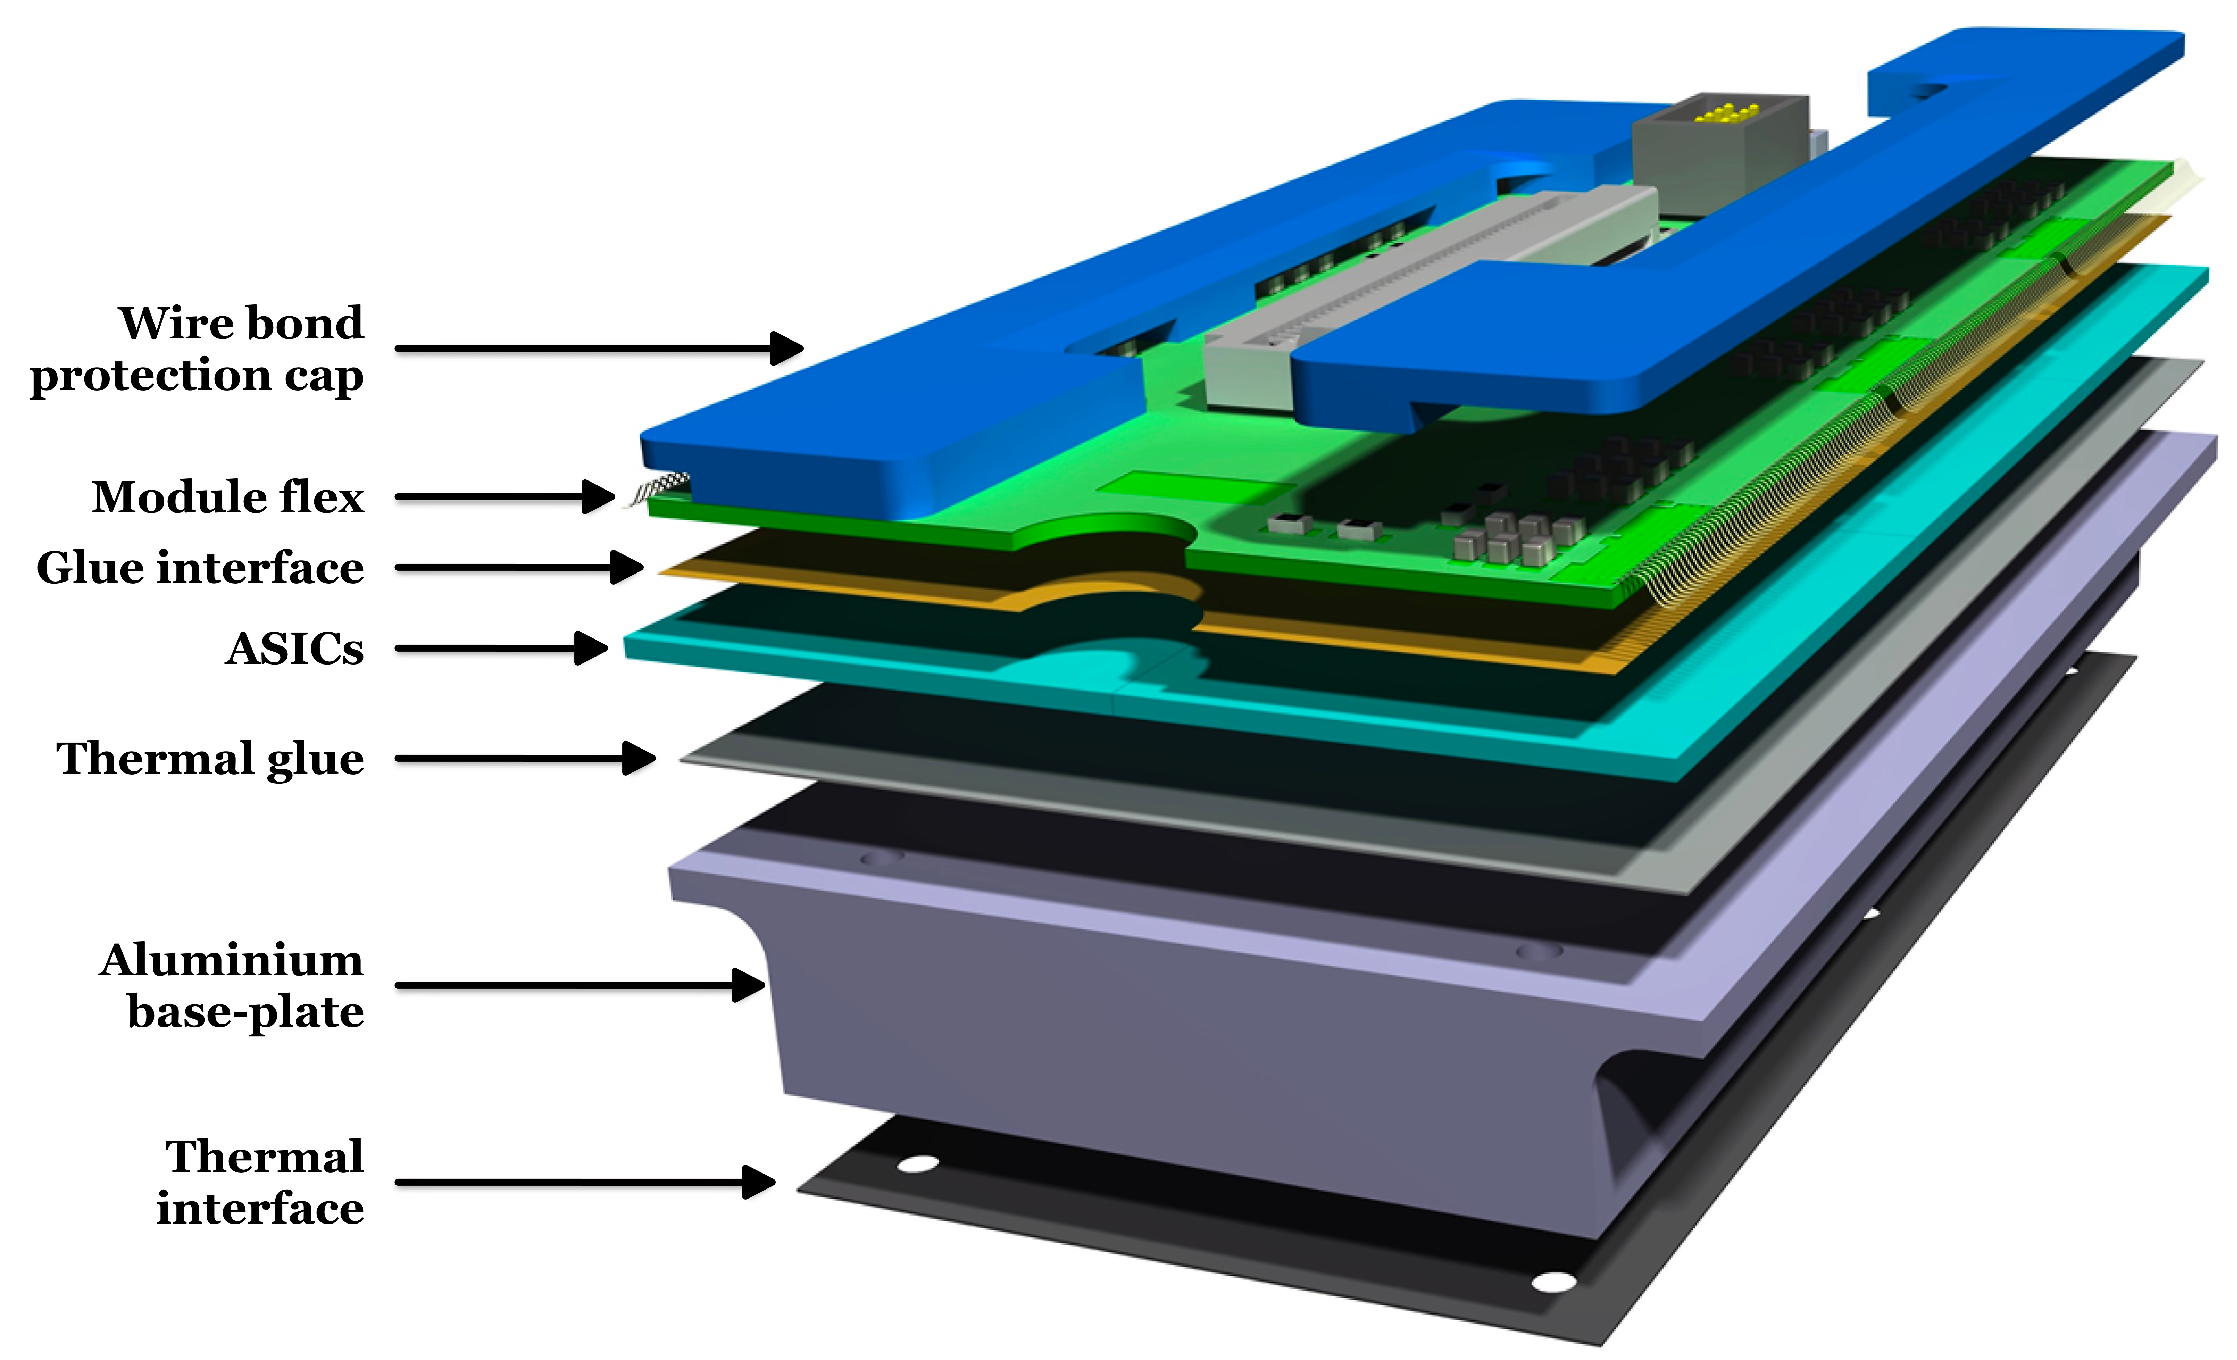
\includegraphics[width=0.7\textwidth]{files/module_CAD}
			\caption{Exploded CAD view of the module. A module is composed by six ASICs glued on an aluminium base-plate. A module flex is glued on top of the module for electrical interconnection. Below the base-plate, a thermal interface sheet is added }
			\label{im:module_CAD}
		\end{figure}
		
		The modules are essentially composed of three distinctives pieces: 
		\begin{enumerate}[i)]
			\item \textbf{The base-plate}: This piece is the back-bone of the ASICs as it mechanical connects them to the rest of the detector. The base-plate is made of aluminium as it provides high thermal conductivity. A thermal interface between the base-plate and the cooling plate as well as thermal glue for the glueing of the ASIC, will be used to ensure a sufficiently good thermal coupling between the cooling plate and the ASICs. The base-plate also receives an electrolytic passivation treatment for electrical surface insulation \cite{PreShower_TP}. \\ There are two types of base-plates, commonly referred to as low-profile and high-profile base-plates, respectively with height of \SI{4}{\milli\meter} and \SI{8}{\milli\meter}. 
			\item \textbf{The ASICs}: They are arranged in a three by two array and are arranged in a specific pattern such that the largest non active periphery part and I/O and powering pads (located at the bottom of Figures \ref{im:ASIC_microscope} and highlighted in \ref{im:prodASIC_floorplan}), are positioned on the edges of the modules. A wise assembly of the modules with a \SI{2}{\milli\meter} overlap, allowed by an alternation of low-profile and high-profile base-plate, provides a reduction of the dead-area at the level of the plane assembly. Figure \ref{im:module_ASIC_only} presents an intermediate step in the assembly of a module (ELECT03) after the ASICs were glued to their base-plate.
			\begin{figure}[h]
				\centering
				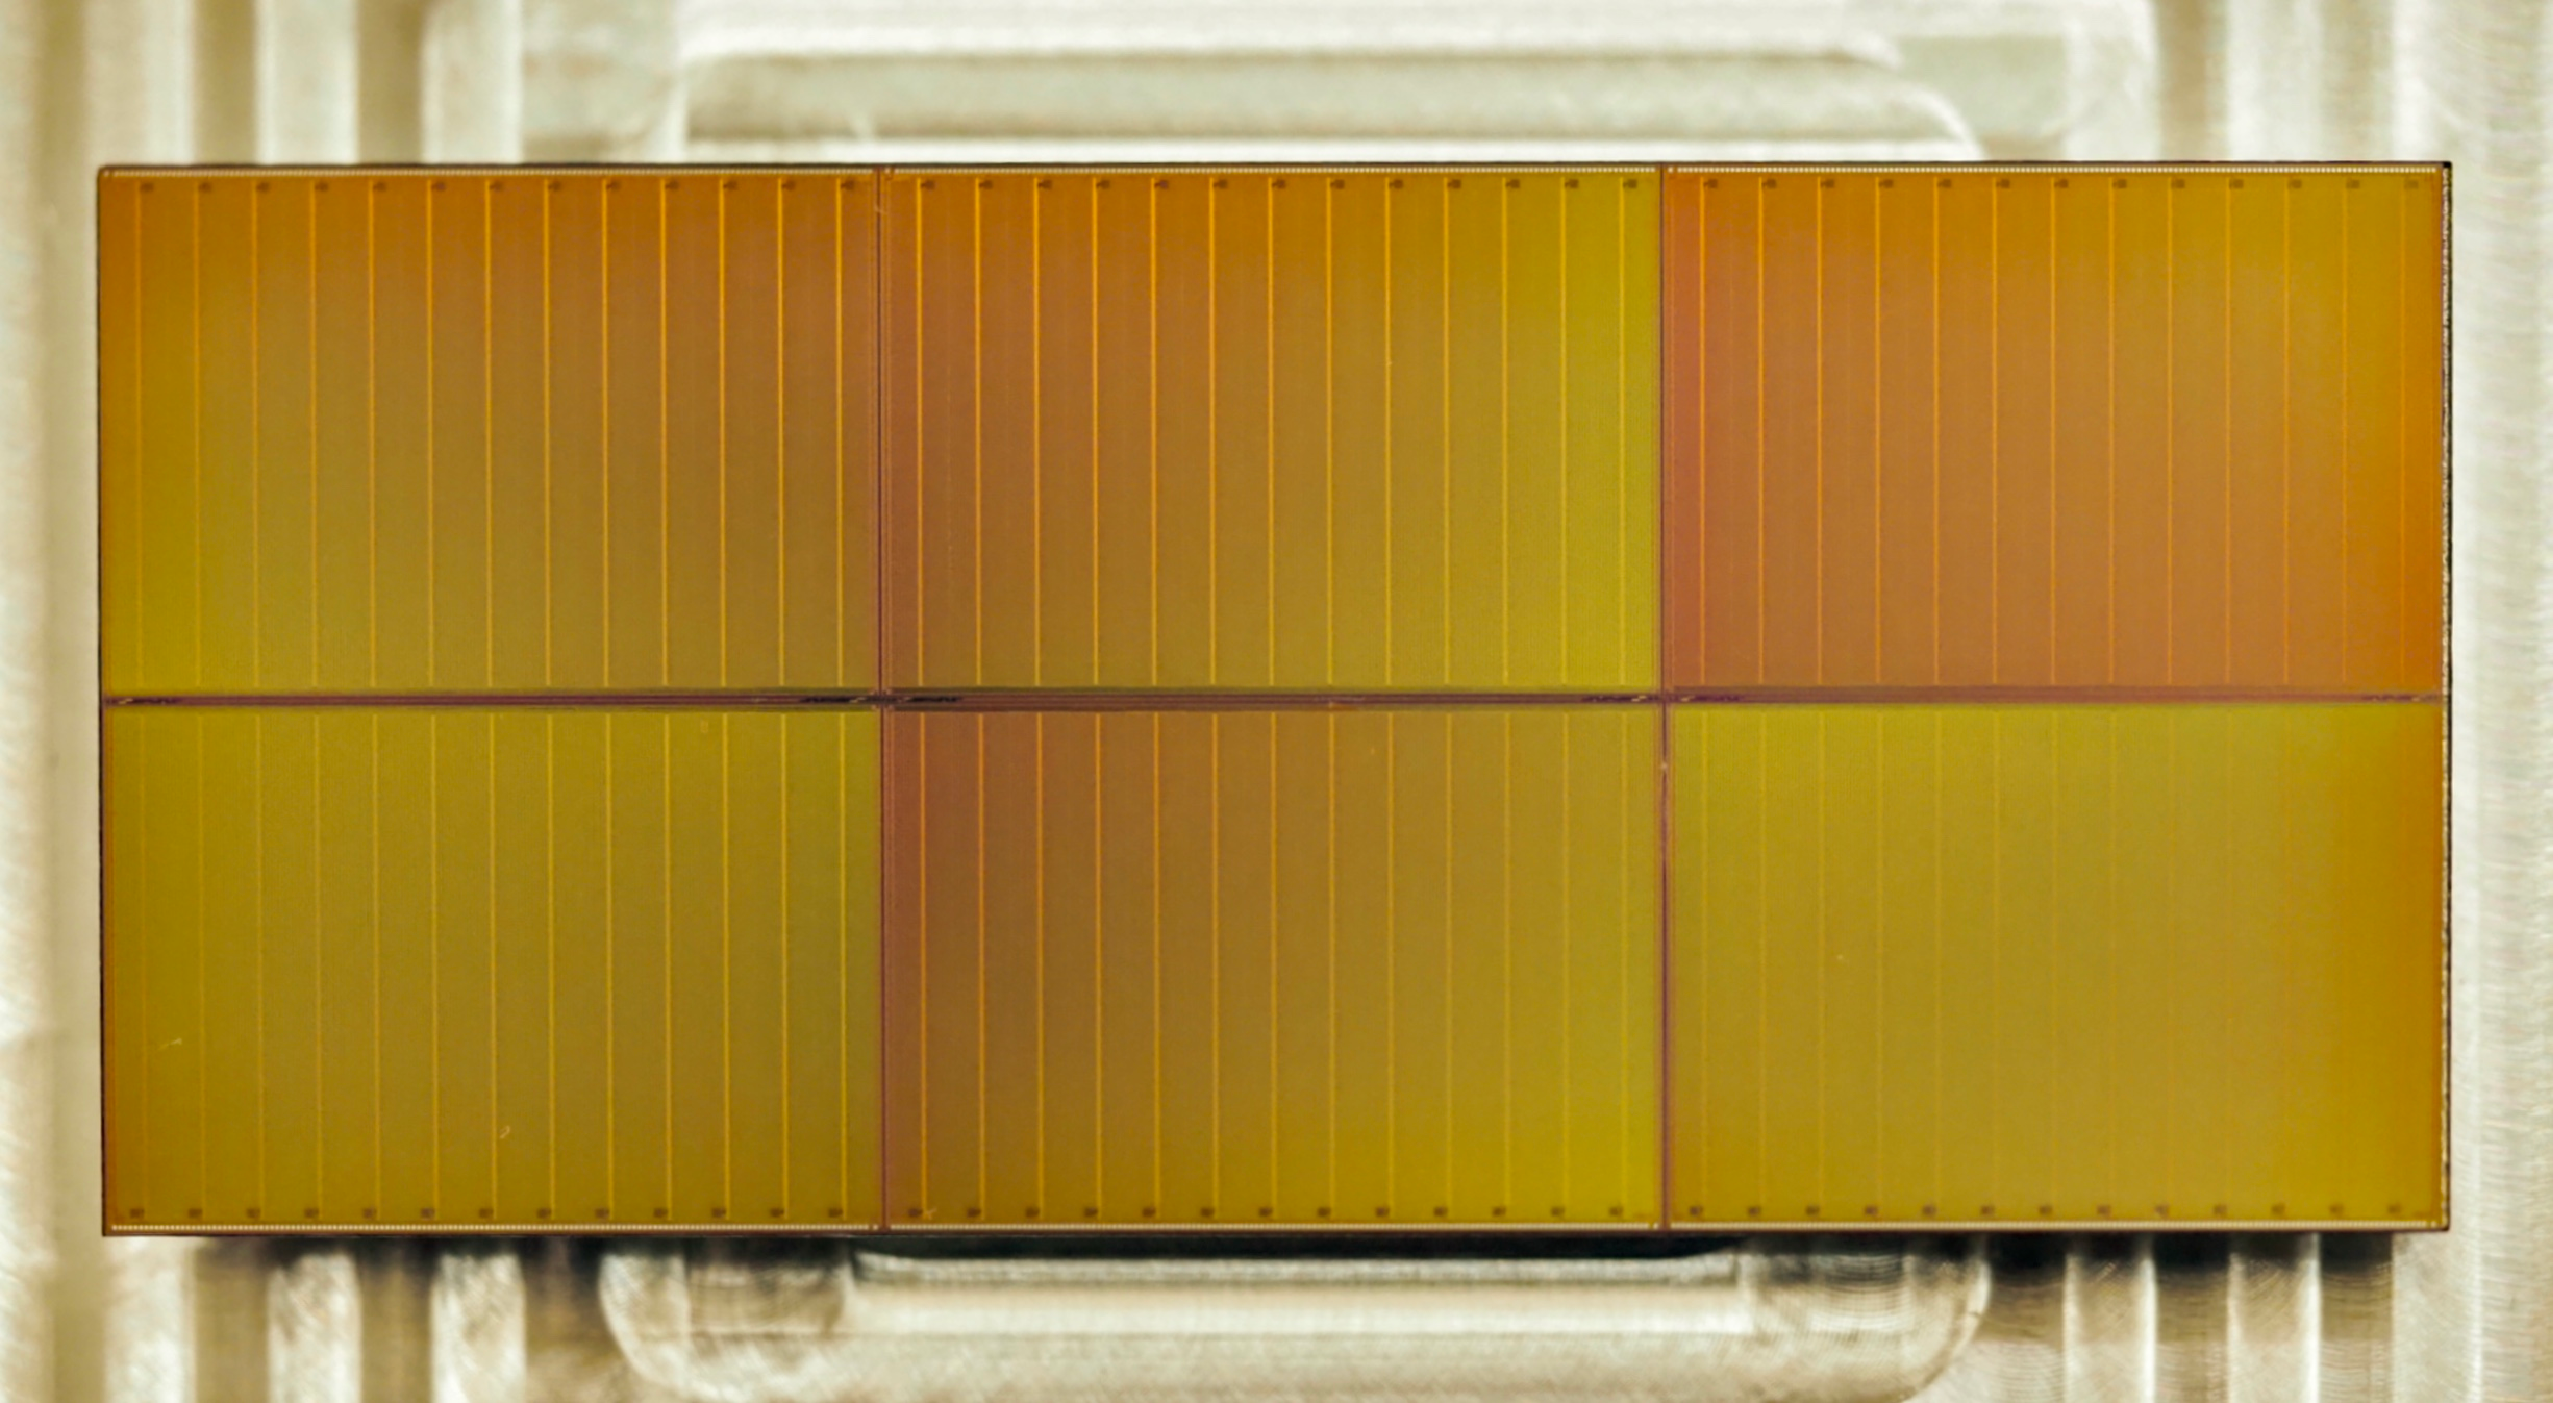
\includegraphics[width=0.8\textwidth]{files/module_ASIC_only}
				\caption{Top view of an intermediary assembly step of modules. Six ASICS are glued to a baseplate such that the part of the ASIC containing the I/O and powering pads and the digital periphery, is located at the top and bottom edges on the module.}
				\label{im:module_ASIC_only}
			\end{figure}
			
			\item \textbf{The module flex}: The electrical interface with the ASICs for I/O and powering is provided by a flexible PCB, glued on top of the ASICs. Figure \ref{im:module_microscope} shows the top view of the module flex after being glued on top of the ASICs and wire-bonding was completed. 
			\begin{figure}[h]
				\centering
				\includegraphics[width=0.8\textwidth]{files/module_microscope}
				\caption{Microscope image of the module flex glued on top of the ASICs after wire-bonding. The central connector is for digital communication while the right connector is for powering.}
				\label{im:module_microscope}
			\end{figure} 
		
			 Each ASICs requires 134 wire-bonds connection to be made between its metallic pads and the metallic lines on the module flex. The module flex has a zero-insertion force connector for the digital signal and a separate pigtail for power lines. The module will drive two low voltages lines, $V_{ccA}$ for the analog part of the ASIC and $V_{dd,dig}$ for the digital part of the ASIC, and a High Voltage line for depletion of the sensor\cite{PreShower_TP}. In order to protect the very sensible wire-bonds, a plastic protection cap is glue on the module flex, giving little clearance for the wire-bonds while protecting them from. A bent wire-bond could create a short and if irreparable or un-noticed, it could compromise an entire module and damage its ASICs. The protection cap will also allow for the powering and communication cables to be laid on top of the modules without damaging the wire-bonds.  
		\end{enumerate} 
		
		The assembly procedure of modules will further be described in \note{section ref}, showing the diverse iterations leading to a more robust and refined procedure. Once 12 modules are assembled, one can build a detector plane. 
		
		\subsection{Detector Planes \textcolor{red}{ 1 pages}}
		The FASER Pre-Shower detector planes consist in an arrangement of two columns and six rows for a total of twelve modules per plane. As anticipated before, there exist two sub-categories of module according to the thickness of the base-plate. Since modules are built such that the largest dead-area region of the ASICs is located on the top and bottom edges, an overlap between modules of \SI{2}{\milli\meter} is used to minimise the dead-area at the level of the entire plane. This is doable only thanks of the \SI{4}{\milli\meter} in height different between low-profile and high-profile base-plates. A side view of the CAD model of the plane with 12 modules mounted on the cooling plate is shown in figure \ref{im:plane_CAD}.
		\begin{figure}[h]
			\centering
			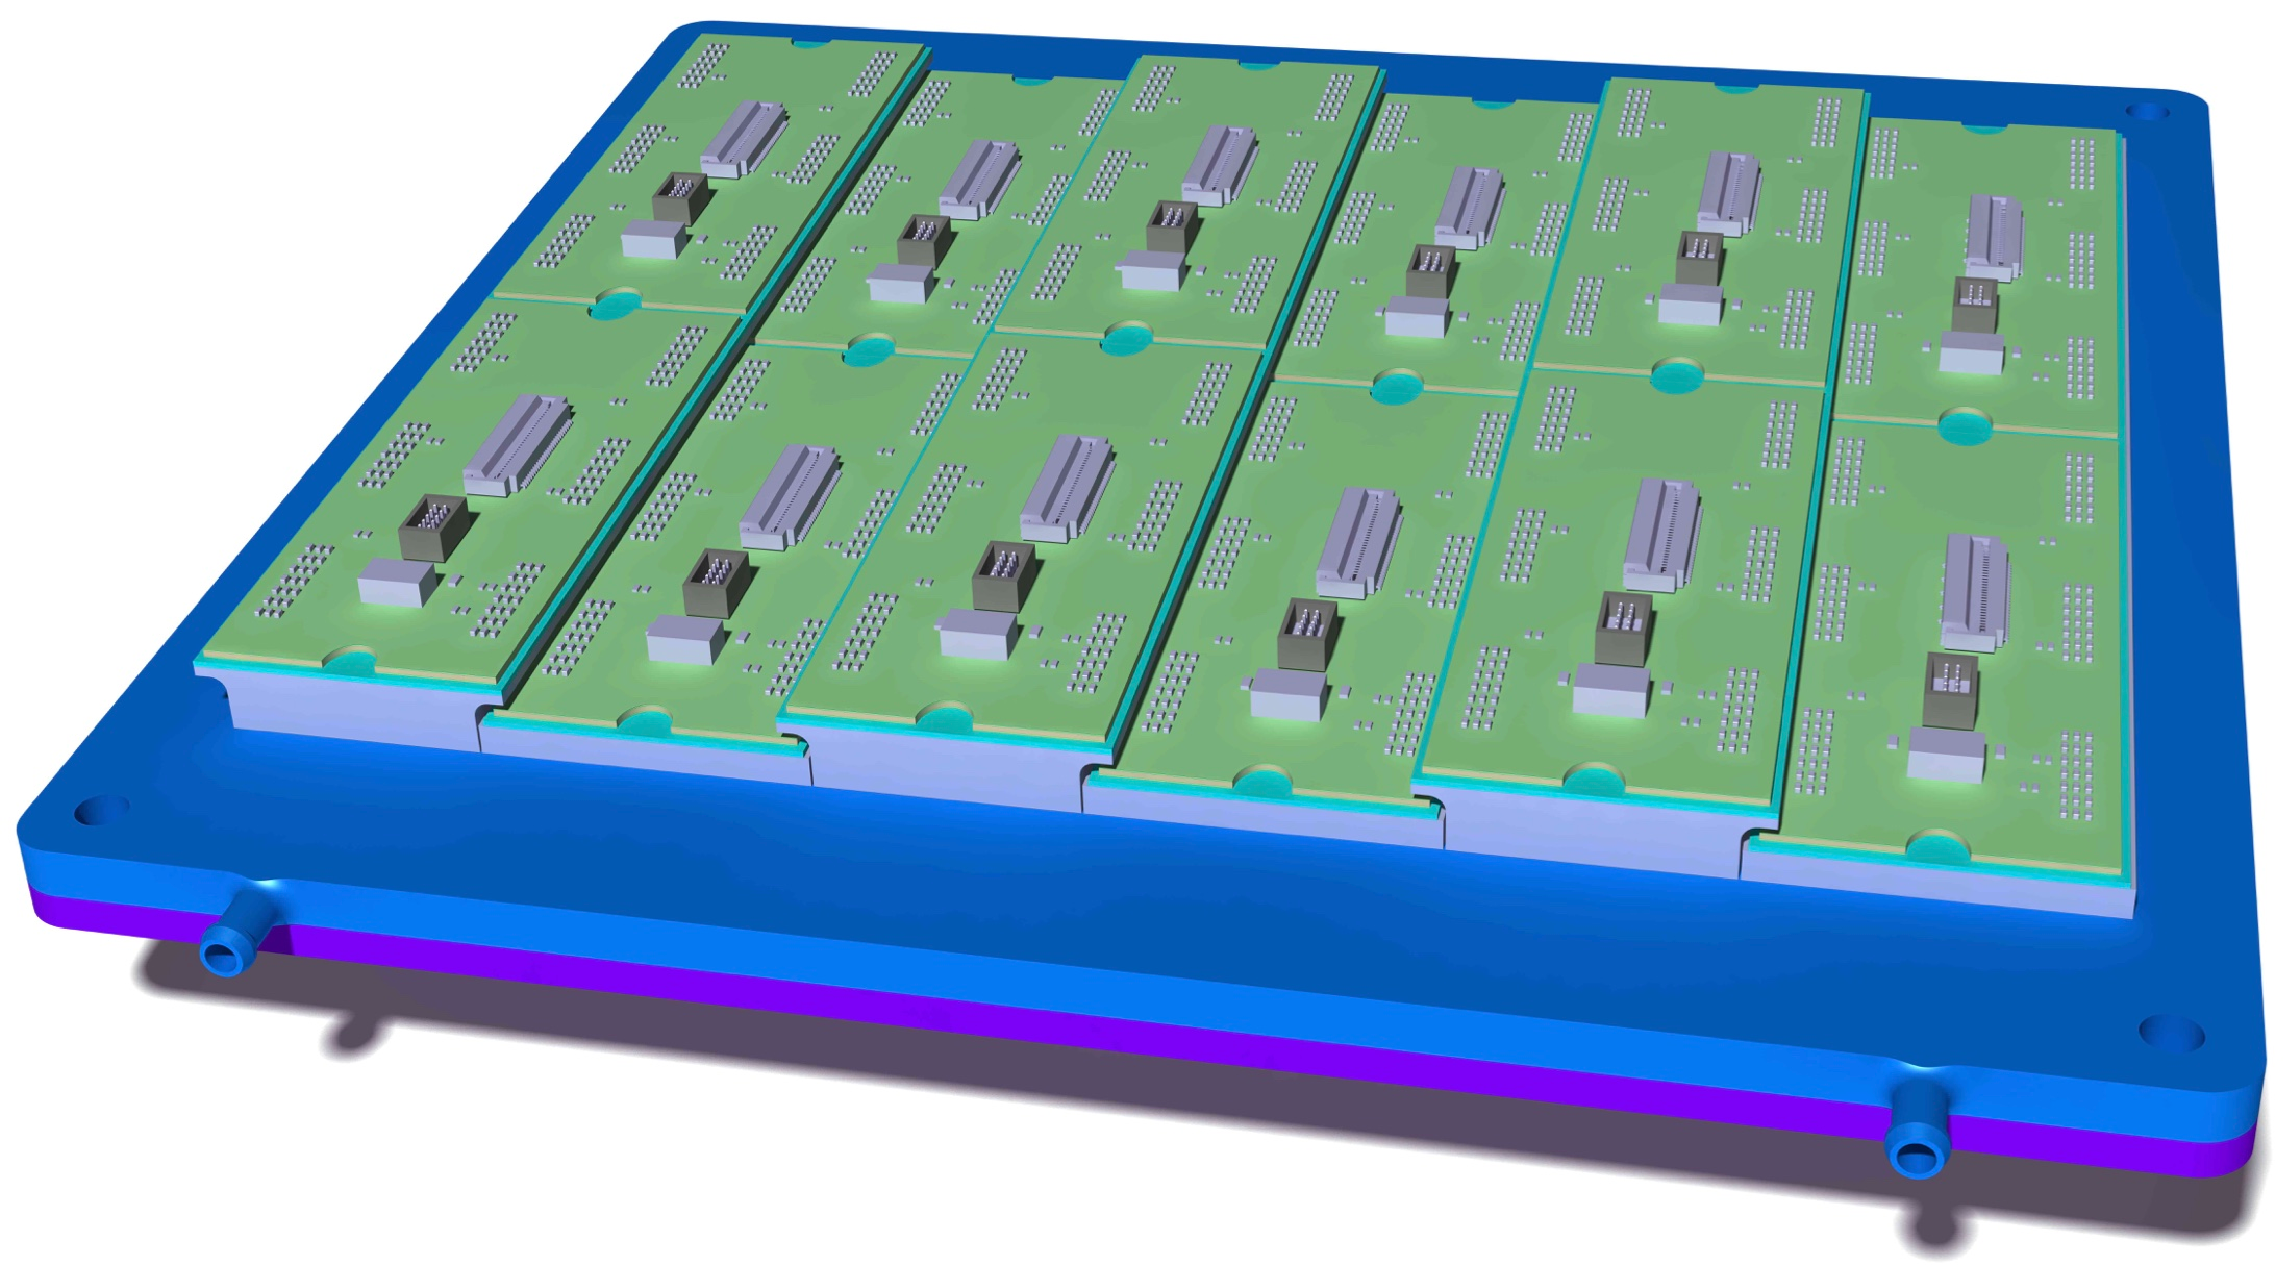
\includegraphics[width=0.8\textwidth]{files/plane_CAD}
			\caption{CAD image of the 12 modules mounted on the cooling plate of the plane. The modules are arranged in two columns of six rows and within a column the low-profile and high-profile modules are alternated with overlap of \SI{2}{\milli\meter}, showing the clearance obtained for the wire-bonds and the protection cap.}
			\label{im:plane_CAD}
		\end{figure}
		
		The active area of the plane, accounting for the overlap of modules, totals 13.4$\times$17.5 cm$^2$. The aperture of the magnets used in the tracking spectrometer represent an area defined by a \SI{10}{\centi\meter} radius circle, the overlap of the activera area and the aperture represent a coverage of 73.2\% from the Pre-Shower. \\
		
		The modules are mounted on a cooling plate used to dissipate the heat produced by the ASICs. The systems is designed to operate at room temperature, which will require a good thermal path between the ASIC and the cooling plate to maintain a temperature below $\sim$ \SI{30}{\celsius}. The tracking stations are already cooled using water as coolant fluid, kept at a temperature of \SI{15}{\celsius} and could hence be used to cool the Pre-Shower planes as well. 
		
		A mock-up set-up was realised to confirm the design, the power transferred to the cooling plate was over-estimated by a 30\%, showing for a a wide range of coolant flows, a temperature increase of not more than \SI{3}{\celsius}. As a result, the planes could be connected in series to each other and the entire Pre-Shower would be connected in series to the tracking stations. For an hypothetical Pre-Shower composed of six detector planes, this would mean a difference in temperature of not more than \SI{4}{\celsius} between the first and sixth plane \cite{PreShower_TP}.
		
		When mounted on the cooling plate, the modules are aligned using precisely drilled holes at the bottom of the base-plates. A metrology survey will be performed after assembly, using precise reference point at the edges of the ASICs, to reconstruct precisely the position of each ASIC, hence each pixel in the Pre-Shower. The coordinates will serve as a basis for the geometry of the reconstruction software but will be fine tuned using track data \cite{PreShower_TP}.
		
		The layers of tungsten radiators are directly integrated in the planes and are located on the opposite side of the cooling plate. Once assembled, the structure is loaded in an aluminium frame serving both for assembly of planes together ans as support for mounting the frame containing the Active Patch Panel (APP) and Logic Board (LB). The volume of the aluminium frame gives enough clearance for the communication and power pigtails to be mounted on top of the modules, running towards the APPs. Each plane is composed of two APPs and two LBs so that each connected to a column of 6 modules in the plane. Figure \ref{im:plane_full} shows the assembly of a Pre-Shower plane with all of the components, including the twelve modules, their communication and powering pigtails, the two APPs and LBs and the humidity and temperature sensors.
		
		\begin{figure}[h]
			\centering
			\includegraphics[width=0.85\textwidth]{files/plane_full}
			\caption{Full Pre-Shower plane assembly. On the left are located the twelve modules, mounted on the cooling plate. The communication pigtail (flat orange) and the powering pigtail (twisted red and white) are connected from the modules to the APP. The right-most module is connected with the shortest pigtails on the left-most slot on the APP and vice versa. A humidity and temperature sensor are located on the bottom right corner of the cooling plate and connected on one of the APPs.}
			\label{im:plane_full}
		\end{figure}
		
		
		
		
		
		 
		
		\subsection{Logic Board and Active Patch Panel}
		
		
		
		
		
		
		\subsection{Layout of the Pre-Shower  \textcolor{red}{ 2 pages}}
% TODO CH5: insert the image of the development of the shower across different detector planes as usually shown in conference. There should be a version in perspective made for the DPNC poster somewhere
		
		
		
		
		
		
		
		
		
		
		
		
		
		
		
		
		
		
		
		
		
		
		
		
		
		
		
		
		
		
		
		
		
		
		
		
		
		
	\clearpage	
	\section{Readout and Detector Control  \textcolor{blue}{ 4 pages}}
		\subsection{Readout \textcolor{red}{ 2 pages}}
		\subsection{Logic Board and APP \textcolor{red}{ 2 pages}}
		\subsection{PIM and Interlock \textcolor{red}{ 2 pages}}
		\subsection{Thermal Cooling}